\documentclass{article}
\usepackage{fancyhdr} % for pretty formatting
\usepackage{amsmath} % for matrices
\usepackage{amssymb} % for bold text
\usepackage{pgfplots} % for graphs
\pgfplotsset{compat=1.18}

\usepackage{lipsum} % For dummy text

\pagestyle{fancy}
\fancyhf{} % Clear all header and footer fields

\lhead{Joshua Dunne}
\rhead{\thepage} % Displays the current page number
\lfoot{MATH620}
\cfoot{Homework 1}

\begin{document}
\section{Question 1}
    \subsection{Consider}
    \begin{center}
    $4 \begin{bmatrix}1 \\ -3 \end{bmatrix}$ and $-2 \begin{bmatrix}3 \\ 5 \end{bmatrix}$
    \end{center}
    \subsection{Graphical representation unscaled}
        \begin{minipage}{0.49\textwidth}
            \centering
            \begin{tikzpicture}
                \begin{axis}[
                    width=\linewidth,
                    title={1, -3},
                    xmin= -7, xmax=7,
                    ymin=-7, ymax=7
                ]
                \addplot[blue, smooth, mark=*] coordinates {
                    (0,0) (1, -3)
                };
                \end{axis}
            \end{tikzpicture}
            \label{fig:graph1}
        \end{minipage}
        \hfill % Add a horizontal space between the graphs
        % Start of second minipage
        \begin{minipage}{0.49\textwidth}
            \centering
            \begin{tikzpicture}
                \begin{axis}[
                    width=\linewidth,
                    title={3, 5},
                    xmin= -7, xmax=7,
                    ymin=-7, ymax=7
                ]
                \addplot[red, smooth, mark=*] coordinates {
                    (0,0) (3,5)
                };
                \end{axis}
            \end{tikzpicture}
        \end{minipage}%
    \subsection{Graphical representation scaled}
        \begin{minipage}{0.49\textwidth}
        \centering
        \begin{tikzpicture}
            \begin{axis}[
                width=\linewidth,
                title={4 * (1, -3)},
                xmin= -13, xmax=13,
                ymin=-13, ymax=13
            ]
            \addplot[blue, smooth, mark=*] coordinates {
                (0,0) (4, -12)
            };
            \end{axis}
        \end{tikzpicture}
    \end{minipage}
    \hfill % Add a horizontal space between the graphs
    % Start of second minipage
    \begin{minipage}{0.49\textwidth}
        \centering
        \begin{tikzpicture}
            \begin{axis}[
                width=\linewidth,
                title={-2 * (3, 5)},
                xmin= -13, xmax=13,
                ymin=-13, ymax=13
            ]
            \addplot[red, smooth, mark=*] coordinates {
                (0,0) (-6,-10)
            };
            \end{axis}
        \end{tikzpicture}
    \end{minipage}%
    \subsection{Changes}
    As can be seen in the graphs above. The coefficient before each of the column
    matrices can be seen to scale any offset. For example, were we to take negative
    one times a matrix, then the offset would extend as far in the negative directions
    as a matrix extended in the positives.
\section{Question 2}
    \subsection{Quick reiteration}
    Having found that we were unable to reach old man Gauss's house using only
    one form of transport, justify this conclusion with two approaches.
    \subsection{First approach}
    \paragraph{Induction}
        For this to be true we'd, much like before, need a coefficient with which
        we'd be able to multiply by our column vector to get to $\begin{bmatrix}107 \\ 64\end{bmatrix}$
        \[{c_1}\begin{bmatrix}3 \\ 1\end{bmatrix} = \begin{bmatrix}107 \\ 64\end{bmatrix}\]
        \[{c_2}\begin{bmatrix}1 \\ 2\end{bmatrix} = \begin{bmatrix}107 \\ 64\end{bmatrix}\]
        However, there simply are not $c_1$ or $c_2$ $\in{\mathbb{R}}$ that satisfy either equation.
        It is therefor impossible to reach his home.
    \subsection{Second approach}
    \paragraph{Visual}
        We can illustrate this as a form of argument. As $\begin{bmatrix}3 \\ 1\end{bmatrix}$ forms a line
        $y=\frac{3}{1}x+0$ That is, by scaling, we can point the end of this vector
        to any point on the line defined. However $(107, 64)$ is not on that line. No possible scaling
        could result in a point that is not on the line.
        \begin{center}
        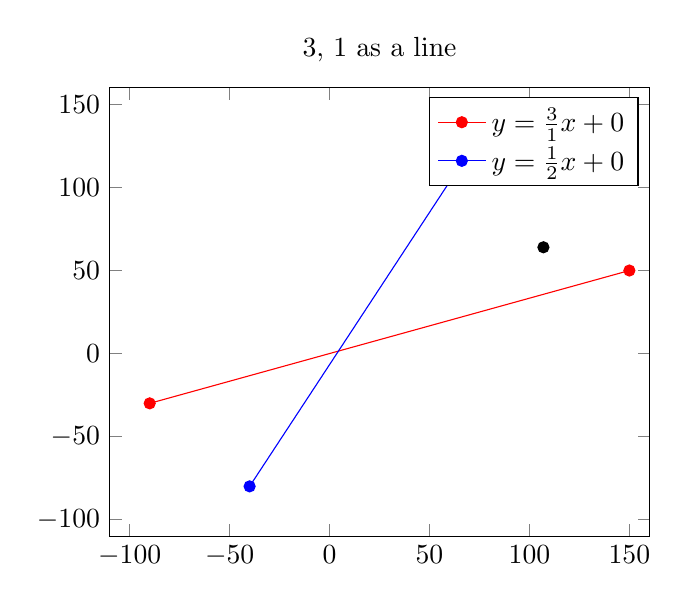
\begin{tikzpicture}
            \begin{axis}[
                title={3, 1 as a line},
                xmin= -110, xmax=160,
                ymin=-110, ymax=160
            ]
            \addplot[red, smooth, mark=*] coordinates { (-90,-30) (150,50) };
            \addlegendentry{$y=\frac{3}{1}x+0$}
            \addplot[blue, smooth, mark=*] coordinates { (-40,-80) (80,140) };
            \addlegendentry{$y=\frac{1}{2}x+0$}
            \addplot[only marks, mark=*] coordinates { (107,64) };
            \end{axis}
        \end{tikzpicture}
        \end{center}
    \paragraph{Analysis}
    As can be seen as depicted, either vector, when scaled, is insufficient
    to reach the point. It is only when we combine the two that we can reach
    both old man Gauss's house and the entirety of $\mathbb{R}^2$
\end{document}